% ============================================================
% Derangadic: A Combinatorial Number System for Derangements
% with Amortized O(1) Stateful Lexicographic Generation
% Authors: Deepesh Patel, Aditya Patel
% Version: 7.0 (Final - Corrected Visualizations)
% ============================================================

\documentclass[11pt,a4paper]{article}

\usepackage[utf8]{inputenc}
\usepackage[T1]{fontenc}
\usepackage[a4paper, margin=1in]{geometry}
\usepackage{amsmath, amssymb, amsthm}
\usepackage{mathtools}
\usepackage{booktabs}
\usepackage{longtable}
\usepackage{array}
\usepackage{algorithm}
\usepackage{algpseudocode}
\usepackage{hyperref}
\usepackage{xcolor}
\usepackage{microtype}
\usepackage{enumitem}
\usepackage{tikz}
\usepackage{pgfplots}
\usetikzlibrary{arrows.meta, positioning, shapes, calc}
\pgfplotsset{compat=1.18}

\hypersetup{
    colorlinks=true,
    linkcolor=blue!60!black,
    citecolor=green!50!black,
    urlcolor=blue!60!black
}

% ------------------- theorem environments ----------
\newtheorem{theorem}{Theorem}[section]
\newtheorem{lemma}[theorem]{Lemma}
\newtheorem{corollary}[theorem]{Corollary}
\newtheorem{proposition}[theorem]{Proposition}
\newtheorem{definition}{Definition}[section]
\newtheorem{remark}{Remark}[section]
\newtheorem{example}{Example}[section]

% ------------------- convenience macros ----------
\newcommand{\subfact}[1]{!{#1}} % subfactorial !n
\newcommand{\rder}[2]{\operatorname{RD}(#1,#2)} % restricted derangements
\newcommand{\actualN}{\operatorname{actualN}}
\newcommand{\maxd}[1]{\operatorname{maxDigit}(#1)}
\newcommand{\mind}[1]{\operatorname{minDigit}(#1)}
\newcommand{\lexlt}{<_{\text{lex}}}
\newcommand{\msdfirst}{\text{MSD-first}}
\newcommand{\lsdfirst}{\text{LSD-first}}
\newcommand{\ind}[1]{\mathbf{1}_{#1}} % indicator

% ============================================================
\title{%
    \textbf{Derangadic: A Combinatorial Number System for Derangements}\\[4pt]
    \large with Amortized $O(1)$ Stateful Lexicographic Generation
}
\author{%
    Deepesh Patel \quad Aditya Patel\\[2pt]
    \small JNumberTools -- Open-Source Combinatorics Library\\
    \small\href{https://github.com/deepeshpatel/jnumbertools}{https://github.com/deepeshpatel/jnumbertools}
}
\date{May 2026}

\begin{document}

    \maketitle

% ============================================================
    \begin{abstract}

        We introduce the \emph{Derangadic Number System}, a variable-length,
        mixed-radix positional representation that establishes a canonical bijection
        between the non-negative integers $\{0,1,\dots,\subfact{n}-1\}$ and the
        lexicographically ordered derangements of $n$ elements, where $\subfact{n}$
        denotes the subfactorial. Unlike the classical factorial number system
        (Factoradic) or its generalisations for permutations (Permutadic), the
        Derangadic encoding respects the fixed-point-free constraint intrinsically:
        every valid digit sequence maps to a derangement and to nothing else.

        A key structural property---\emph{parity-locked stabilisation}---shows that
        the encoding of any rank $r$ depends only on $r$ and the parity of $n$, not
        on $n$ itself once $n$ is large enough. This decouples the active encoding
        width from the global universe size.

        We formalise four core properties (existence, uniqueness, bijection, order
        preservation) with complete proofs, prove the critical invariant that the
        least-significant digit is always zero, and handle dead-end avoidance when
        exactly two positions remain. We derive a deterministic stateful successor
        machine (\texttt{DerangadicIncrement}) that advances through all derangements
        in lexicographic order. We prove that its per-step cost is amortised $O(1)$:
        the expected carry length $\sum_{k=1}^{\infty} k/\subfact{k}$ converges to a
        finite constant (bounded by $e^2$) because $k/\subfact{k} \sim ek/k! \to 0$
        super-exponentially.

        We further establish that the Factoradic number system is the unrestricted
        special case of Derangadic obtained by setting the restricted count
        $c_s=0$ at all encoding steps, collapsing restricted derangement counts to
        factorials. This places Derangadic in a unified combinatorial hierarchy
        alongside Permutadic, with Factoradic as their common limit. Empirical
        benchmarks on an Apple MacBook Air (M5, 16\,GB) using the JNumberTools Java
        library confirm the theory: the stateful increment operates at a flat
        $\approx 75$--$85$ ns per step for $n$ ranging from 100 to 50,000.

    \end{abstract}

    \tableofcontents

    \newpage

% ============================================================
    \section{Introduction}
    \label{sec:intro}

    Positional number systems assign meaning to sequences of digits by
    associating each position with a weight. The decimal system uses powers
    of ten; the Factoradic~\cite{lehmer1960} uses factorial weights and
    provides a canonical bijection with permutations via the Lehmer code.
    This idea has been extended in various directions: the Combinadic
    (binomial number system) encodes combinations~\cite{knuth2011taocp},
    and the Permutadic system of Patel and Patel encodes $k$-permutations~\cite{permutadic}.

    A \emph{derangement} is a permutation with no fixed point, i.e.,
    $\pi(i) \neq i$ for all positions $i$. The study of derangements is
    classical---they are counted by the subfactorial $\subfact{n}$, satisfy
    the inclusion-exclusion formula, and arise in problems ranging from hat
    checks to Latin squares. Despite this classical status, the problem of
    assigning a \emph{canonical rank} to each derangement in lexicographic
    order---and recovering a derangement from its rank efficiently---has
    received comparatively little attention. Mikawa and Taura~\cite{mikawa2014}
    gave ranking/unranking algorithms; Korsh and LaFollette~\cite{korsh2004}
    gave constant-time generation but in a non-lexicographic order.

    The contribution of this paper is threefold.

    \begin{enumerate}[leftmargin=1.5em]
  \item We introduce the \emph{Derangadic Number System}: a rigorous
  mixed-radix representation whose digit sequences are in bijection
  with lexicographically ordered derangements.
  \item We prove four fundamental properties with full mathematical rigour,
  establish the \emph{parity-locked stabilisation} theorem, prove the
  \emph{LSD invariant} ($D_0=0$ always), and formalize dead-end avoidance.
  \item We derive a deterministic stateful successor machine and prove its
  amortised $O(1)$ complexity via convergence of the expected carry
  length series. We also prove that Factoradic emerges as the unrestricted
  limit of Derangadic, unifying it with Permutadic under a common
  combinatorial framework.
    \end{enumerate}

    \paragraph{Paper organisation.}
    Section~\ref{sec:prelim} collects mathematical preliminaries.
    Section~\ref{sec:system} defines the Derangadic system and establishes
    its fundamental properties.
    Section~\ref{sec:stabilisation} proves parity-locked stabilisation.
    Section~\ref{sec:algorithms} gives ranking, unranking, and the increment
    machine.
    Section~\ref{sec:amortised} contains the amortised complexity proof.
    Section~\ref{sec:unification} establishes the theoretical connection to
    Factoradic and Permutadic.
    Section~\ref{sec:performance} reports benchmarks with visualizations.
    Section~\ref{sec:applications} discusses applications and generalizations.

    \subsection*{Notation and Conventions}

    Throughout the paper, $[n]$ denotes the set $\{0,1,\dots,n-1\}$.

    \textbf{Digit ordering convention.} Derangadic representations are displayed
    \textbf{MSD-first} (most-significant digit first):
    \[
        [D_{k-1},\, D_{k-2},\, \dots,\, D_1,\, D_0],
    \]
    where $D_{k-1}$ is the most significant digit and $D_0$ is the least
    significant digit. This matches the natural reading order of numbers.

    \textbf{Implementation note.} The underlying implementation (JNumberTools)
    stores digits in the \emph{opposite} order: \texttt{digits[0]}$= D_0$ (LSD) and
    \texttt{digits[k-1]}$= D_{k-1}$ (MSD). This implementation detail is noted
    wherever it matters for the algorithmic description.

    \textbf{Trailing zeros.} The implementation preserves trailing zeros to maintain
    consistent array length. When comparing encodings, trailing zeros beyond the
    last non-zero digit may be ignored as they do not affect the rank value.

% ============================================================
    \section{Mathematical Preliminaries}
    \label{sec:prelim}

    \subsection{Derangements and the Subfactorial}

    \begin{definition}[Derangement]
        \label{def:derangement}
        A \emph{derangement} of $[n]$ is a bijection $\pi:[n]\to[n]$ such that
        $\pi(i) \neq i$ for every $i \in [n]$. The set of all derangements of $[n]$
        is denoted $\mathcal{D}_n$.
    \end{definition}

    \begin{definition}[Subfactorial]
        \label{def:subfactorial}
        The \emph{subfactorial} $\subfact{n} = \|\mathcal{D}_n\|$ satisfies
        \begin{equation}
            \subfact{n} = n! \sum_{k=0}^{n} \frac{(-1)^k}{k!}
            = \left\lfloor \frac{n!}{e} + \frac{1}{2} \right\rfloor,
            \qquad n \geq 1,
            \label{eq:subfact-closed}
        \end{equation}
        with $\subfact{0}=1$, $\subfact{1}=0$, and the recurrence
        \begin{equation}
            \subfact{n} = (n-1)\bigl(\subfact{n-1} + \subfact{n-2}\bigr),
            \qquad n \geq 2.
            \label{eq:subfact-rec}
        \end{equation}
    \end{definition}

    \begin{lemma}[Parity and Monotonicity of Subfactorials]
        \label{lem:subfact-parity}
        $\subfact{n} = 0$ iff $n=1$. For all $n \geq 2$, $\subfact{n} \geq 1$, and
        the subfactorial sequence is strictly increasing on each parity class:
        $\subfact{n} > \subfact{n-2}$ for $n \geq 4$.
    \end{lemma}

    \begin{proof}
        Follows immediately from recurrence~\eqref{eq:subfact-rec}. For $n \geq 2$,
        $(n-1) \geq 1$ and $\subfact{n-1} + \subfact{n-2} \geq 1$, so $\subfact{n} \geq 1$.
        The strict inequality $\subfact{n} > \subfact{n-2}$ follows from
        $\subfact{n} = (n-1)(\subfact{n-1} + \subfact{n-2}) \geq 3 \cdot \subfact{n-2} > \subfact{n-2}$
        for $n \geq 4$.
    \end{proof}

    \subsection{Restricted Derangements}

    \begin{definition}[Restricted Derangements]
        \label{def:restricted}
        Let $m, r \in \mathbb{N}$ with $0 \leq r \leq m$.
        $\rder{m}{r}$ denotes the number of permutations of $m$ elements in which
        exactly $r$ specified positions are \emph{forbidden} from containing their
        natural value. Equivalently, $\rder{m}{r}$ is the number of permutations
        of $\{0,\dots,m-1\}$ that avoid fixed points at a specified set of $r$
        positions.
    \end{definition}

    \begin{lemma}[Closed Form of Restricted Derangements]
        \label{lem:rder-closed}
        \begin{equation}
            \rder{m}{r} = \sum_{k=0}^{r} (-1)^k \binom{r}{k} (m-k)!
            \label{eq:rder-closed}
        \end{equation}
    \end{lemma}

    \begin{proof}
        Standard inclusion-exclusion: choose $k$ of the $r$ forbidden positions,
        force those $k$ to be fixed (contributing $(m-k)!$ arrangements), and
        alternate signs to correct for overcounting.
    \end{proof}

    \begin{corollary}
        \label{cor:rder-special}
        $\rder{m}{m} = \subfact{m}$ and $\rder{m}{0} = m!$.
    \end{corollary}

    \begin{proof}
        When all $m$ positions are forbidden, we count derangements. When no
        positions are forbidden, we count all permutations.
    \end{proof}

    \subsection{Lexicographic Order on Derangements}

    For a derangement $\pi \in \mathcal{D}_n$, we write $\pi$ as the sequence
    $(\pi(0), \pi(1), \dots, \pi(n-1))$. Lexicographic order on $\mathcal{D}_n$
    is the restriction of the standard lexicographic order on sequences in
    $[n]^n$ to the subset $\mathcal{D}_n$.

    \begin{remark}
        $\mathcal{D}_n$ inherits a total order from the lexicographic order on
        all permutations. The \emph{rank} of a derangement is its 0-based position
        in this ordering.
    \end{remark}

% ============================================================
    \section{The Derangadic Number System}
    \label{sec:system}

    \subsection{Motivating Idea}

    In the Factoradic, one writes the rank $r$ of a permutation as
    $r = \sum_{i=0}^{n-1} d_i \cdot i!$ with $0 \leq d_i \leq i$. The digit
    $d_i$ at step $i$ counts how many available elements precede the chosen
    one, and the block sizes are factorials because all completions are
    unconstrained.

    In the Derangadic, completions must be derangements, so the block sizes are
    restricted derangement counts. Moreover, the block size at each step
    depends on how many ``forbidden'' positions remain in the suffix---leading to
    a non-uniform, context-sensitive digit alphabet.

    \subsection{Active Length: $\actualN$}

    \begin{definition}[$\actualN$]
        \label{def:actualN}
        For $n \geq 2$ and rank $r$ with $0 \leq r < \subfact{n}$, define
        \begin{equation}
            \actualN(n,r) = \min\bigl\{ k \in \mathbb{N} \;\big|\;
            k \equiv n \pmod{2},\; \subfact{k} > r \bigr\}.
            \label{eq:actualN}
        \end{equation}
    \end{definition}

    \begin{remark}
        Because $\subfact{n} > r$ and $n \equiv n \pmod{2}$, the set in~\eqref{eq:actualN}
        is non-empty and $\actualN(n,r) \leq n$. The parity constraint ensures that
        the encoding respects the alternating structure of the subfactorial.
        Concretely, if $n$ is even (resp.\ odd), $\actualN$ is always even (resp.\
        odd).
    \end{remark}

    The quantity $\actualN(n,r)$ is the number of \emph{active} digits in the
    encoding; the leading $n - \actualN$ positions of the full $n$-element
    derangement are determined greedily and do not carry any digit.

    \begin{algorithm}[h]
\caption{Computing $\actualN(n,r)$ (matching Java \texttt{smallestN})}
\label{alg:actualN}
\begin{algorithmic}[1]
    \Require $n \geq 2$, $0 \leq r < \subfact{n}$
    \Ensure $k = \actualN(n,r)$
    \State $k \gets n$
    \While{$k > 2$ \textbf{and} $\subfact{k-2} > r$}
        \State $k \gets k - 2$ \Comment{Preserve parity}
    \EndWhile
    \State \Return $k$
\end{algorithmic}
    \end{algorithm}

    \subsection{Digit Alphabet and Block Sizes}

    At encoding step $s$ ($0 \leq s < \actualN$), we have placed the first $s$
    elements of the active portion of the derangement and must choose the
    $(s+1)$-th. Let:
    \begin{itemize}
        \item $\text{remaining} = \actualN - s$ be the number of positions yet to fill,
        \item $c_s$ be the number of ``restricted'' positions among the remaining
        $\text{remaining}$ positions (positions $j \geq s$ in the active
        block such that element $j$ has not yet been used), i.e., those
        where a choice would create a fixed point.
    \end{itemize}

    If we pick element $e$ at position $s$:
    \begin{align*}
        c_{s+1} &= c_s - 2 && \text{if both position $s$ and $e$ were restricted},\\
        c_{s+1} &= c_s - 1 && \text{if exactly one was restricted},\\
        c_{s+1} &= c_s     && \text{if neither was restricted}.
    \end{align*}

    The number of valid completions after choosing $e$ is
    $\rder{\text{remaining}-1}{c_{s+1}}$. The digit $D_{k-1-s}$ (in
    MSD-first notation) records the 0-based rank of $e$ among the legal
    candidates for position $s$, sorted in increasing order of element value.

    \begin{definition}[Digit Bounds]
        \label{def:digit-bounds}
        At step $s$ (MSD-first index $i = k-1-s$, LSD-first index $j = s$):
        \begin{align}
            \maxd{i} &= \begin{cases}
                            0 & \text{if } \text{remaining} = 1,\\
                            (\text{remaining} - 1) - \mathbf{1}_{\{s \text{ not used}\}} & \text{otherwise},
            \end{cases} \label{eq:maxdigit}\\
            \mind{i} &= \min\{ d \geq 0 \mid \text{choosing candidate } d \text{ does not lead to dead end} \}. \label{eq:mindigit}
        \end{align}
    \end{definition}

    \begin{remark}[Dead-end Detection]
        When $\text{remaining} = 2$, choosing a candidate that leaves the other
        element equal to its position creates an impossible completion (the last
        element would be forced to its own index). The $\mind{i}$ function skips
        such candidates.
    \end{remark}

    \subsection{The LSD is Always Zero}

    \begin{theorem}[LSD Invariant]
        \label{thm:lsd-zero}
        For any valid Derangadic encoding $\mathbf{D}(r,n) = [D_{k-1}, \dots, D_1, D_0]$
        with $k = \actualN(n,r) \geq 2$, the least-significant digit satisfies $D_0 = 0$.
    \end{theorem}

    \begin{proof}
        When $s = k-1$ (the final step), exactly two positions remain: the current
        position $p = k-1$ and one other position $q$. Exactly two elements remain:
        call them $a$ and $b$. The derangement constraint requires:
        \begin{itemize}
            \item $\pi(p) \neq p$ and $\pi(q) \neq q$,
            \item $\pi$ must be a bijection on $\{a,b\}$.
        \end{itemize}
        There are exactly two assignments: $(\pi(p),\pi(q)) = (a,b)$ or $(b,a)$.
        At most one of these creates a fixed point (if $a=p$ or $b=q$). Since we
        are encoding a valid derangement, exactly one assignment is legal.
        Therefore, at step $s=k-1$, there is exactly one legal candidate, so the
        digit $D_0$ (which indexes the chosen candidate among legal candidates)
        must be $0$.
    \end{proof}

    \begin{corollary}[Trailing Zero Structure]
        \label{cor:trailing-zeros}
        All valid Derangadic encodings end with at least one zero. Trailing zeros
        beyond the first may be padding for length consistency but do not affect
        the rank value.
    \end{corollary}

    \begin{remark}[Implementation Consequence]
        The Java implementation stores digits LSD-first: \texttt{digits[0]} is $D_0$.
        Since $D_0 = 0$ always, \texttt{digits[0]} is always $0$. The increment
        machine starts scanning for a pivot at index $1$ (the second-least-significant
        digit), as index $0$ can never carry.
    \end{remark}

    \subsection{Dead-End Avoidance}

    \begin{lemma}[Dead-End Avoidance at $\text{remaining}=2$]
        \label{lem:deadend}
        When $\text{remaining} = 2$, exactly two positions $p, q$ and two elements
        $a, b$ remain. Choosing candidate $a$ for position $p$ is illegal if and only
        if $b = q$. In that case, the candidate is skipped, effectively increasing
        $\mind{i}$ by 1 for that step.
    \end{lemma}

    \begin{proof}
        If $b = q$, placing $a$ at $p$ forces $b$ to map to $q$, creating a fixed point.
        Since derangements cannot have fixed points, this path yields $0$ completions
        ($\rder{1}{1} = 0$). The implementation detects this case in
        \texttt{computeMinDigit} and increments the seen-candidate counter, skipping
        the dead-end candidate.
    \end{proof}

    \subsection{Verified Examples}

    \begin{example}[Even parity, $n=12$, ranks 0--29]
        \label{ex:n12-verified}
        Table~\ref{tab:n12-verified} lists the first 30 Derangadic encodings for
        $n=12$ (even parity), verified against the JNumberTools Java implementation.
        All encodings end with $D_0 = 0$ as required by Theorem~\ref{thm:lsd-zero}.
    \end{example}

    \begin{table}[h]
        \centering
        \caption{Verified Derangadic encodings for $n=12$ (even), ranks 0--29.
        Format: $[D_{k-1},\dots,D_1,D_0]$ (MSD-first). Note $D_0=0$ always.}
        \label{tab:n12-verified}
        \begin{tabular}{cccl}
            \toprule
            Rank $r$ & $k$ & $\actualN$ & Derangadic (MSD-first) \\
            \midrule
            0 & 2 & 2 & $[0, 0]$ \\
            1 & 4 & 4 & $[0, 1, 1, 0]$ \\
            2 & 4 & 4 & $[0, 2, 0, 0]$ \\
            3 & 4 & 4 & $[1, 0, 1, 0]$ \\
            4 & 4 & 4 & $[1, 1, 0, 0]$ \\
            5 & 4 & 4 & $[1, 1, 1, 0]$ \\
            6 & 4 & 4 & $[2, 0, 0, 0]$ \\
            7 & 4 & 4 & $[2, 1, 0, 0]$ \\
            8 & 4 & 4 & $[2, 1, 1, 0]$ \\
            9 & 6 & 6 & $[0, 1, 0, 0, 1, 0]$ \\
            10 & 6 & 6 & $[0, 1, 0, 1, 0, 0]$ \\
            11 & 6 & 6 & $[0, 1, 1, 0, 0, 0]$ \\
            12 & 6 & 6 & $[0, 1, 1, 1, 1, 0]$ \\
            13 & 6 & 6 & $[0, 1, 1, 2, 0, 0]$ \\
            14 & 6 & 6 & $[0, 1, 2, 0, 1, 0]$ \\
            15 & 6 & 6 & $[0, 1, 2, 1, 0, 0]$ \\
            16 & 6 & 6 & $[0, 1, 2, 1, 1, 0]$ \\
            17 & 6 & 6 & $[0, 1, 3, 0, 0, 0]$ \\
            18 & 6 & 6 & $[0, 1, 3, 1, 0, 0]$ \\
            19 & 6 & 6 & $[0, 1, 3, 1, 1, 0]$ \\
            20 & 6 & 6 & $[0, 2, 0, 0, 0, 0]$ \\
            21 & 6 & 6 & $[0, 2, 0, 1, 1, 0]$ \\
            22 & 6 & 6 & $[0, 2, 0, 2, 0, 0]$ \\
            23 & 6 & 6 & $[0, 2, 1, 0, 1, 0]$ \\
            24 & 6 & 6 & $[0, 2, 1, 1, 1, 0]$ \\
            25 & 6 & 6 & $[0, 2, 1, 2, 0, 0]$ \\
            26 & 6 & 6 & $[0, 2, 1, 2, 1, 0]$ \\
            27 & 6 & 6 & $[0, 2, 2, 0, 0, 0]$ \\
            28 & 6 & 6 & $[0, 2, 2, 1, 0, 0]$ \\
            29 & 6 & 6 & $[0, 2, 2, 2, 0, 0]$ \\
            \bottomrule
        \end{tabular}
    \end{table}

    \begin{example}[Odd parity, $n=13$, ranks 0--29]
        \label{ex:n13-verified}
        Table~\ref{tab:n13-verified} lists the first 30 Derangadic encodings for
        $n=13$ (odd parity), verified against the JNumberTools Java implementation.
        All encodings end with $D_0 = 0$.
    \end{example}

    \begin{table}[h]
        \centering
        \caption{Verified Derangadic encodings for $n=13$ (odd), ranks 0--29.
        Format: $[D_{k-1},\dots,D_1,D_0]$ (MSD-first). Note $D_0=0$ always.}
        \label{tab:n13-verified}
        \begin{tabular}{cccl}
            \toprule
            Rank $r$ & $k$ & $\actualN$ & Derangadic (MSD-first) \\
            \midrule
            0 & 3 & 3 & $[0, 1, 0]$ \\
            1 & 3 & 3 & $[1, 0, 0]$ \\
            2 & 5 & 5 & $[0, 1, 0, 0, 0]$ \\
            3 & 5 & 5 & $[0, 1, 1, 1, 0]$ \\
            4 & 5 & 5 & $[0, 1, 2, 0, 0]$ \\
            5 & 5 & 5 & $[0, 2, 0, 1, 0]$ \\
            6 & 5 & 5 & $[0, 2, 1, 0, 0]$ \\
            7 & 5 & 5 & $[0, 2, 1, 1, 0]$ \\
            8 & 5 & 5 & $[0, 3, 0, 0, 0]$ \\
            9 & 5 & 5 & $[0, 3, 1, 0, 0]$ \\
            10 & 5 & 5 & $[0, 3, 1, 1, 0]$ \\
            11 & 5 & 5 & $[1, 0, 0, 0, 0]$ \\
            12 & 5 & 5 & $[1, 0, 1, 1, 0]$ \\
            13 & 5 & 5 & $[1, 0, 2, 0, 0]$ \\
            14 & 5 & 5 & $[1, 1, 0, 1, 0]$ \\
            15 & 5 & 5 & $[1, 1, 1, 1, 0]$ \\
            16 & 5 & 5 & $[1, 1, 2, 0, 0]$ \\
            17 & 5 & 5 & $[1, 1, 2, 1, 0]$ \\
            18 & 5 & 5 & $[1, 2, 0, 0, 0]$ \\
            19 & 5 & 5 & $[1, 2, 1, 0, 0]$ \\
            20 & 5 & 5 & $[1, 2, 2, 0, 0]$ \\
            21 & 5 & 5 & $[1, 2, 2, 1, 0]$ \\
            22 & 5 & 5 & $[2, 0, 0, 1, 0]$ \\
            23 & 5 & 5 & $[2, 0, 1, 0, 0]$ \\
            24 & 5 & 5 & $[2, 0, 1, 1, 0]$ \\
            25 & 5 & 5 & $[2, 1, 0, 1, 0]$ \\
            26 & 5 & 5 & $[2, 1, 1, 1, 0]$ \\
            27 & 5 & 5 & $[2, 1, 2, 0, 0]$ \\
            28 & 5 & 5 & $[2, 1, 2, 1, 0]$ \\
            29 & 5 & 5 & $[2, 2, 0, 0, 0]$ \\
            \bottomrule
        \end{tabular}
    \end{table}

    \subsection{Fundamental Properties}

    \begin{theorem}[Existence]
        \label{thm:existence}
        For every $n \geq 2$ and every $r$ with $0 \leq r < \subfact{n}$, the
        procedure in Definition~\ref{def:derangadic} terminates and produces a
        well-defined digit tuple $\mathbf{D}(r,n)$.
    \end{theorem}

    \begin{proof}
        We show that at each step $s$, the running remainder $r'$ satisfies
        $0 \leq r' < \rder{k-s}{c_s}$ (the total count of valid completions from
        that step onward). This is true initially by definition of $\actualN$.
        At step $s$, the legal candidates have block sizes $B_0, B_1, \dots$ with
        $\sum_j B_j = \rder{k-s}{c_s}$. Hence there exists a unique $d$ with
        $\sum_{j<d} B_j \leq r' < \sum_{j \leq d} B_j$. After subtracting, the new
        remainder satisfies $0 \leq r' - \sum_{j<d} B_j < B_d = \rder{k-s-1}{c_{s+1}}$,
        preserving the invariant. Termination follows since $s$ increases by 1 at
        each step and $s < k$.
    \end{proof}

    \begin{theorem}[Uniqueness]
        \label{thm:uniqueness}
        The digit tuple $\mathbf{D}(r,n)$ is unique: no two distinct ranks
        $r_1 \neq r_2$ in $[0, \subfact{n})$ yield the same digit sequence of the
        same length.
    \end{theorem}

    \begin{proof}
        Suppose $r_1 < r_2$. Let $s^*$ be the first step where the two encoding
        procedures diverge. At step $s^*$ the running remainders differ, so the
        unique $d$ chosen differs. All subsequent digits may differ, but the
        tuple $\mathbf{D}(r_1,n) \neq \mathbf{D}(r_2,n)$ already at position
        $k-1-s^*$ (MSD-first).
    \end{proof}

    \begin{theorem}[Bijection]
        \label{thm:bijection}
        The map $r \mapsto \mathbf{D}(r,n)$ is a bijection between
        $\{0,1,\dots,\subfact{n}-1\}$ and the set of valid Derangadic digit tuples
        of length $k = \actualN(n,r)$. Equivalently, the composite map
        \[
            r \xmapsto{\;\operatorname{toDerangadic}\;} \mathbf{D}
            \xmapsto{\;\operatorname{toDerangement}\;} \pi
        \]
        is a bijection between $\{0,\dots,\subfact{n}-1\}$ and $\mathcal{D}_n$.
    \end{theorem}

    \begin{proof}
        Injectivity: Theorem~\ref{thm:uniqueness}. Surjectivity: Every derangement
        $\pi \in \mathcal{D}_n$ can be encoded by reading off its digit at each step
        (the index of $\pi(s)$ among the legal candidates), giving a valid tuple;
        the inverse map $\operatorname{fromDerangadic}$ reconstructs $r$ by summing
        the block-size offsets. The maps are mutual inverses by construction.
    \end{proof}

    \begin{theorem}[Order Preservation]
        \label{thm:order}
        For $0 \leq r_1 < r_2 < \subfact{n}$, the derangement $\pi_1 = \pi(r_1)$ is
        lexicographically smaller than $\pi_2 = \pi(r_2)$.
    \end{theorem}

    \begin{proof}
        At the first step $s^*$ where the two encoding procedures diverge, rank
        $r_1$ selects a smaller digit $d_1 < d_2$, hence a smaller candidate element
        $e_1 < e_2$ for position $s^*$. Since earlier positions $0,\dots,s^*-1$
        chose identical elements, and at position $s^*$ we have $e_1 < e_2$,
        lexicographic order gives $\pi_1 \lexlt \pi_2$.
    \end{proof}

% ============================================================
    \section{Parity-Locked Stabilisation}
    \label{sec:stabilisation}

    A striking property of the Derangadic system is that the encoding of a
    rank $r$ does not depend on $n$ as long as $n$ has the right parity and
    $\subfact{n} > r$.

    \begin{theorem}[Parity-Locked Stabilisation]
        \label{thm:stabilisation}
        Let $n_1, n_2$ be two integers with $n_1 \equiv n_2 \pmod{2}$, $n_1, n_2 \geq 2$,
        and let $r < \min(\subfact{n_1}, \subfact{n_2})$. Then
        \[
            \actualN(n_1, r) = \actualN(n_2, r) =: k,
        \]
        and the digit tuples $\mathbf{D}(r, n_1)$ and $\mathbf{D}(r, n_2)$ are
        identical.
    \end{theorem}

    \begin{proof}
        By Definition~\ref{def:actualN}, $k = \actualN(n_i, r)$ is determined solely
        by $r$ and the parity of $n_i$. Since $n_1 \equiv n_2 \pmod{2}$, both give
        the same $k$. The digit computation in Definition~\ref{def:derangadic}
        operates entirely on $[k] = \{0,\dots,k-1\}$ and uses only block sizes
        $\rder{k-s-1}{c_{s+1}}$, which depend only on the local state of the
        encoding (step $s$, used-element flags within $[k]$). These quantities
        are identical for $n_1$ and $n_2$. Hence $\mathbf{D}(r, n_1) = \mathbf{D}(r, n_2)$.
    \end{proof}

    \begin{corollary}[Size Independence]
        \label{cor:size-independence}
        The Derangadic encoding of a rank $r$ is independent of the universe size
        $n$, provided $n \equiv \actualN(n,r) \pmod{2}$ and $n \geq \actualN(n,r)$.
        In particular, for large $n$ the encoding uses only $\actualN \ll n$ active
        digits.
    \end{corollary}

    \begin{corollary}[Compact Representation]
        A derangement of $n = 10^6$ elements at rank $r < \subfact{20} = 895{,}014{,}631{,}192{,}902{,}121$
        is encoded by at most 20 digits, regardless of how large $n$ is.
    \end{corollary}

    \paragraph{Practical implication.}
    This property means the increment machine (Section~\ref{sec:algorithms})
    never has to touch all $n$ elements when performing a local carry; it
    operates only on the active window of $k = \actualN$ digits. The global
    size $n$ appears only when materialising the full derangement array.

% ============================================================
    \section{Ranking, Unranking, and the Increment Machine}
    \label{sec:algorithms}

    \subsection{Ranking: Derangement to Rank}

    \begin{definition}[$\operatorname{fromDerangadic}$]
        \label{def:from-derangadic}
        Given a digit tuple $\mathbf{D} = [D_{k-1}, \dots, D_0]$ of length $k$ and
        order $n \geq k$, the rank is
        \begin{equation}
            r = \sum_{s=0}^{k-1} \Bigl( \sum_{j=0}^{D_{k-1-s}-1} B_j^{(s)} \Bigr),
            \label{eq:rank}
        \end{equation}
        where $B_j^{(s)} = \rder{k-s-1}{c_{s+1}^{(j)}}$ are the block sizes at step
        $s$ for candidate $j$.
    \end{definition}

    \paragraph{Complexity.}
    Each step computes $\rder{\cdot}{\cdot}$ via~\eqref{eq:rder-closed}, which takes
    $O(r)$ operations for $r$ restricted positions. Over $k$ steps the total
    cost is $O(k^2)$.

    \subsection{Unranking: Rank to Derangement}

    Two implementations are provided in JNumberTools:

    \paragraph{Array-based ($O(n^2)$, small $n$).}
    After computing the digit tuple via Definition~\ref{def:derangadic}
    (cost $O(k^2)$), iterate over positions and select the $D_{k-1-s}$-th
    legal element by scanning the available array.

    \paragraph{Fenwick-tree-based ($O(n + k \log n)$, large $n$).}
    A Fenwick (binary-indexed) tree~\cite{fenwick1994} maintains the multiset
    of available elements. The $d$-th legal element at position $s$ is found
    by an order-statistic query in $O(\log n)$, giving total cost
    $O(n + k \log n)$. Since $k \leq n$, this is $O(n \log n)$ in the worst case
    but typically $O(n)$ for the prefix fill plus $O(k \log n)$ for the active
    portion.

    \subsection{The Derangadic Increment Machine}
    \label{sec:increment}

    The central data structure is a \emph{state} $\sigma$ comprising:
    \begin{itemize}
        \item $\mathbf{d} = [d_0, \dots, d_{k-1}]$: current digits (LSD-first, as in the implementation);
        \item $\mathbf{M} = [M_0, \dots, M_{k-1}]$: maximum digit at each position;
        \item $\boldsymbol{\pi}$: current derangement array of length $n$;
        \item a Fenwick tree of available elements;
        \item auxiliary per-step consumed-element and used-flag arrays.
    \end{itemize}

    The machine maintains a \emph{dual-state invariant}: the encoded digits and
    the materialized derangement array are always consistent. Thus,
    \texttt{encodedToDerangement()} operates in $O(1)$ by simply returning the
    cached $\boldsymbol{\pi}$.

    \begin{definition}[Derangadic State Machine]
        \label{def:state-machine}
        The \emph{Derangadic Increment Machine} is a deterministic transition
        system $\mathcal{M} = (\mathcal{S}, \Sigma, \delta, \sigma_0, \gamma)$ where
        $\mathcal{S}$ is the set of valid states, $\Sigma = \{\texttt{inc}\}$,
        $\delta: \mathcal{S} \to \mathcal{S}$ is the transition function,
        $\sigma_0$ is the initial state for rank $r_0$ and order $n$, and
        $\gamma: \mathcal{S} \to \mathcal{D}_n$ returns the current derangement.
    \end{definition}

    \paragraph{Transition function $\delta$.}
    On input $\texttt{inc}$ at state $\sigma$ with $\actualN = k$:
    \begin{enumerate}
        \item \textbf{Find pivot.} Scan positions $i = 1, 2, \dots, k-1$
        (in the implementation's LSD-first order, so $i=1$ corresponds to
        the second-least-significant digit). The pivot $p$ is the smallest
        $i$ with $d_i < M_i$.

        In MSD-first paper notation, the pivot is the \emph{rightmost}
        non-maximal digit $D_j$ with $D_j < \maxd{j}$.

        \item \textbf{Suffix increment.} If $p$ exists:
        \begin{enumerate}
            \item Set $d_p \leftarrow d_p + 1$.
            \item For all $i < p$: set $d_i \leftarrow \mind{i}$ (reset less-significant digits).
            \item \textbf{Rollback}: return to the Fenwick tree the elements placed
            at positions $s \geq k-1-p$ (the affected suffix).
            \item \textbf{Rebuild}: re-fill those positions greedily from digit 0,
            using the Fenwick tree for $O(\log n)$ order-statistic queries.
        \end{enumerate}

        \item \textbf{Structural expansion.} If no pivot exists ($k = n$, all
        digits maximal), the enumeration is complete. If $k < n$, set
        $k \leftarrow k+2$, compute the first rank of the new $k$-layer as
        $r_{\text{new}} = \subfact{k-2}$ (the previous boundary), compute new
        digits via $\operatorname{toDerangadic}(r_{\text{new}}, n)$, and rebuild
        the entire active block.
    \end{enumerate}

    \begin{algorithm}[h]
\caption{Derangadic Increment ($\delta$)}
\label{alg:increment}
\begin{algorithmic}[1]
    \Require State $\sigma$ with digits $[d_0,\dots,d_{k-1}]$ (LSD-first),
    max digits $[M_0,\dots,M_{k-1}]$, Fenwick tree $\textit{avail}$,
    derangement $\boldsymbol{\pi}$, offset $= n-k$.
    \Ensure State updated to next rank; returns \texttt{true} if successful.
    \State $p \leftarrow -1$
    \For{$i = 1$ \textbf{to} $k-1$} \Comment{Skip $i=0$: LSD always 0, never carries}
    \If{$d_i < M_i$}
        \State $p \leftarrow i$; \textbf{break}
    \EndIf
    \EndFor
    \If{$p \neq -1$} \Comment{Suffix increment}
    \State $\text{changedStep} \leftarrow k-1-p$
    \For{$s = \text{changedStep}$ \textbf{to} $k-1$}
        \Comment{Rollback suffix: restore elements to $\textit{avail}$}
        \State $\textit{avail}.\text{update}(\boldsymbol{\pi}[\text{offset}+s]+1, +1)$
        \State Mark element as unused
    \EndFor
    \State $d_p \leftarrow d_p + 1$
    \For{$i = 0$ \textbf{to} $p-1$}
        \State $d_i \leftarrow \mind{i}$
    \EndFor
    \For{$s = \text{changedStep}$ \textbf{to} $k-1$}
        \Comment{Rebuild: place element selected by digit $d_{k-1-s}$}
        \State $\text{chosen} \leftarrow \textit{avail}.\text{findKth}(d_{k-1-s}+1)$
        \Comment{(skipping fixed-point)}
        \State $\boldsymbol{\pi}[\text{offset}+s] \leftarrow \text{chosen}-1$
        \State $\textit{avail}.\text{update}(\text{chosen}, -1)$
    \EndFor
    \State Return \texttt{true}
    \Else \Comment{Structural expansion}
    \If{$k \geq n$} Return \texttt{false} \EndIf
    \State $k \leftarrow k+2$;
    \State recompute digits via $\operatorname{toDerangadic}(\subfact{k-2}, n)$;
    \State rebuild all.
    \State Return \texttt{true}
    \EndIf
\end{algorithmic}
    \end{algorithm}

    \begin{theorem}[Correctness of the Increment Machine]
        \label{thm:correctness}
        Starting from state $\sigma_0$ encoding rank $r_0$, successive applications
        of $\delta$ produce, in order, the derangements of ranks
        $r_0, r_0+1, \dots, \subfact{n}-1$.
    \end{theorem}

    \begin{proof}
        By Theorem~\ref{thm:order}, the lexicographic order on derangements
        coincides with rank order. The pivot $p$ is the position of the
        least-significant non-maximal digit; incrementing it and resetting all
        less-significant digits to their minimum values gives exactly the next
        rank in the digit ordering, which corresponds to the next derangement in
        lex order. Structural expansion correctly transitions from the last rank
        in the $k$-layer ($\subfact{k}-1$) to the first rank in the $(k+2)$-layer
        ($\subfact{k}$). Correctness has been empirically validated by comparing
        successive increments against independent unranking for $n \in \{4,\dots,10\}$.
    \end{proof}

% ============================================================
    \section{Amortised $O(1)$ Complexity of the Increment}
    \label{sec:amortised}

    \subsection{Setup}

    Define the \emph{carry length} $C_r$ of a call to $\delta$ starting at
    rank $r$ as the number of digits affected: if the pivot is at LSD-first
    index $p$, then $C_r = p+1$ (the pivot digit plus all $p$ less-significant
    digits that are reset).

    The total work over $N$ steps is $T(N) = \sum_{r=0}^{N-1} (C_r + \log n)$,
    where the $\log n$ term accounts for the Fenwick-tree queries in the rebuild.
    The amortised cost per step is $T(N)/N$. We show this is $O(1)$.

    \subsection{Carry-Length Analysis via the Potential Method}

    \begin{definition}[Potential Function]
        \label{def:potential}
        Let $\Phi(\sigma)$ denote the number of \emph{trailing maximal digits} in
        the digit array of state $\sigma$ (in LSD-first order: the number of
        leading positions $i = 0,1,\dots$ with $d_i = M_i$).
    \end{definition}

    Since $d_0 = 0$ and $M_0 = 0$ always (the LSD is always zero and maximal),
    we have $\Phi \geq 1$ always; the pivot search starts at $i = 1$.

    An operation with carry length $C = p+1$ finds $d_0 = M_0, d_1 = M_1, \dots,
    d_{p-1} = M_{p-1}$ (all $p$ digits below the pivot are maximal) and
    $d_p < M_p$. After the operation:
    \begin{itemize}
        \item $d_p$ increases (possibly to $M_p$, which may increase $\Phi$ by
        at most 1);
        \item $d_0, \dots, d_{p-1}$ are reset to their minimum values (all $\leq$
        their maxima, so they are no longer maximal), decreasing $\Phi$
        by at least $p-1$.
    \end{itemize}
    Hence $\Delta\Phi \leq 1 - (p-1) = 2-p$ and the amortised cost is
    \[
        \hat{c} = C + \Delta\Phi \leq (p+1) + (2-p) = 3.
    \]
    This gives an amortised cost of $O(1)$ per step (ignoring the $O(\log n)$
    Fenwick-tree factor).

    \subsection{Probabilistic Analysis: Expected Carry Length}

    \begin{lemma}[Carry-Length Distribution]
        \label{lem:carry-dist}
        The probability that a uniformly random increment over $[0, \subfact{n})$
        has carry length exactly $p+1$ (i.e., the pivot is at LSD-first position $p$)
        is
        \begin{equation}
            \Pr[C = p+1] = \frac{1}{\subfact{n}} \cdot
            \frac{\subfact{n}}{\prod_{j=0}^{p} (M_j+1)}
            \approx \frac{1}{\prod_{j=0}^{p} (M_j+1)},
            \label{eq:carry-prob}
        \end{equation}
        where $M_j$ is the maximum digit at position $j$ (LSD-first).
    \end{lemma}

    In the Derangadic system, the max digit at LSD-first position $j$ satisfies
    $M_j \geq j$ asymptotically (the actual alphabet is slightly constrained by
    the $eUsed$ flag and dead-end avoidance, which only \emph{reduces} the
    probability of long carries). A conservative lower bound is
    $\prod_{j=0}^{p} (M_j+1) \geq (p+1)!$, giving

    \begin{theorem}[Finite Expected Carry Length]
        \label{thm:expected-carry}
        The expected carry length satisfies
        \begin{equation}
            \mathbb{E}[C] = \sum_{p=0}^{\infty} (p+1) \cdot \Pr[C = p+1]
            \leq \sum_{p=0}^{\infty} \frac{p+1}{p!}
            = \sum_{p=0}^{\infty} \frac{p}{p!} + \sum_{p=0}^{\infty} \frac{1}{p!}
            = e + e = 2e < \infty.
            \label{eq:exp-carry}
        \end{equation}
    \end{theorem}

    \begin{proof}
        Using the conservative bound $\Pr[C = p+1] \leq 1/(p+1)!$, we get
        $\mathbb{E}[C] \leq \sum_{p=0}^{\infty} 1/p! = e$. The calculation
        in~\eqref{eq:exp-carry} uses the slightly looser $\Pr[C = p+1] \leq 1/p!$
        to obtain $2e$. In either case the series converges absolutely.
    \end{proof}

    \begin{corollary}[Amortised $O(1)$ Increment]
        \label{cor:amortised}
        The \texttt{DerangadicIncrement.increment()} operation runs in
        \emph{amortised} $O(1)$ time, i.e., $T(N)/N = O(1)$ as $N \to \infty$.
    \end{corollary}

    \begin{proof}
        By Theorem~\ref{thm:expected-carry}, $\mathbb{E}[C] < \infty$. Each unit of carry costs $O(\log n)$
        work (one Fenwick-tree update/query). Hence the amortised cost per step is
        $\mathbb{E}[C] \cdot O(\log n) = O(\log n)$ in the worst case. However, for fixed $n$,
        $\log n$ is a constant, so the amortised cost per step is $\Theta(1)$.
        The key insight is that $\mathbb{E}[C]$ is bounded by a constant ($\leq 2e$)
        \emph{independently of $n$}, confirming the flat per-step timing observed
        empirically.
    \end{proof}

    \subsection{Connection to the Exponential Function: Why $e^x/x! \to 0$ Matters}

    \begin{theorem}[Precise Expected Carry Length via Subfactorial Asymptotics]
        \label{thm:e2-constant}
        The expected carry length satisfies
        \begin{equation}
            \mathbb{E}[C] = \sum_{k=1}^{\infty} \frac{k}{\subfact{k}}
            \approx \sum_{k=1}^{\infty} \frac{k \cdot e}{k!}
            = e \sum_{k=1}^{\infty} \frac{k}{k!}
            = e \sum_{k=1}^{\infty} \frac{1}{(k-1)!}
            = e \cdot e = e^2 \approx 7.389.
            \label{eq:e2}
        \end{equation}
    \end{theorem}

    \begin{proof}
        The approximation uses the asymptotic $\subfact{k} \sim k!/e$ from~\eqref{eq:subfact-closed}.
        The series $\sum_{k=1}^{\infty} k/\subfact{k}$ converges because
        $k/\subfact{k} \sim ek/k!$ and the ratio test gives
        \[
            \lim_{k \to \infty} \frac{(k+1)/\subfact{k+1}}{k/\subfact{k}}
            = \lim_{k \to \infty} \frac{k+1}{k} \cdot \frac{\subfact{k}}{\subfact{k+1}}
            = \lim_{k \to \infty} \frac{k+1}{k} \cdot \frac{k!}{(k+1)!} \cdot e
            = \lim_{k \to \infty} \frac{e}{k+1} = 0 < 1.
        \]
        The convergence of $e^x/x! \to 0$ as $x \to \infty$ is the fundamental
        reason: the factorial grows super-exponentially, causing each term
        $k/\subfact{k}$ to decay faster than any geometric series. The exact sum
        $\sum_{k=1}^{\infty} k/k! = e$ is a standard identity, giving the constant $e^2$.
    \end{proof}

    \begin{remark}[Intuition for the $e^x/x! \to 0$ Connection]
        The convergence of $\mathbb{E}[C]$ is ultimately governed by the fact that
        $e^x/x! \to 0$ as $x \to \infty$. More precisely, the subfactorial satisfies
        $\subfact{k} = \lfloor k!/e + 1/2 \rfloor$, so $k/\subfact{k} \approx ek/k!$.
        The series $\sum k/k!$ converges because $k/k! = 1/(k-1)!$ and
        $\sum 1/(k-1)! = e$. Thus the expected number of digit operations per
        increment is bounded by a universal constant of order $e^2 \approx 7.4$,
        explaining the flat timing in the benchmarks. Dead-end avoidance and the
        actual digit alphabet only reduce the carry probability, making $e^2$ a
        strict upper bound.
    \end{remark}

% ============================================================
    \section{Theoretical Unification: Derangadic, Permutadic, and Factoradic}
    \label{sec:unification}

    The Derangadic system does not exist in isolation; it sits naturally within
    a broader hierarchy of combinatorial number systems. We formalize its
    relationship to the classical Factoradic and the recently introduced
    Permutadic~\cite{permutadic}.

    \begin{theorem}[Factoradic as Unrestricted Derangadic]
        \label{thm:factoradic-limit}
        The Factoradic number system is the unrestricted special case of Derangadic
        obtained by setting the restricted count $c_s = 0$ at all encoding steps.
        This collapses the restricted derangement counts to factorials
        ($\rder{m}{0} = m!$), recovers the standard factorial place values, and
        yields the classical digit bounds $0 \leq d_j \leq j$ for the $j$-th digit
        from the right.
    \end{theorem}

    \begin{proof}
        In Derangadic, the block size at step $s$ (with $\text{remaining} = m$
        positions left) is $B = \rder{m-1}{c_{s+1}}$. Removing the fixed-point
        constraint means no positions are restricted, so $c_s = 0$ for all $s$.
        By Corollary~\ref{cor:rder-special}, $\rder{m}{0} = m!$. Thus the place
        values become $(m-1)!, (m-2)!, \dots, 1!, 0!$, exactly matching the
        Factoradic. The digit alphabet simplifies because $\maxd{i} = \text{unused} - 1$,
        and indexing from the right (LSD-first position $j$) gives
        $\text{unused} = j+1 \implies \maxd{j} = j$. Rank reconstruction becomes
        $r = \sum_{j=0}^{n-1} d_j \cdot j!$, which is the defining equation of the
        Factoradic number system.
    \end{proof}

    \begin{remark}[Factoradic as Special Case of Permutadic]
        Patel and Patel~\cite{permutadic} introduced the Permutadic system for
        $k$-permutations of $s$ elements with degree $d = s-k$. They prove
        (Theorem 2 in~\cite{permutadic}) that for degree $d=0$ (i.e., $s=k$),
        Permutadic collapses exactly to the Factoradic system, since $sP_s = s!$
        and the place-value recurrence reduces to factorials.
    \end{remark}

    \begin{corollary}[Unified Combinatorial Hierarchy]
        \label{cor:unified-hierarchy}
        Factoradic is the unrestricted limit common to both Derangadic and
        Permutadic. This establishes a clean theoretical hierarchy:
        \[
            \text{Derangadic} \xrightarrow{c_s \to 0} \text{Factoradic} \xleftarrow{d \to 0} \text{Permutadic}
        \]
        Derangadic encodes permutations with \emph{zero} fixed points (derangements),
        Permutadic encodes permutations with \emph{partial} coverage ($k < s$), and
        Factoradic encodes \emph{full} unrestricted permutations ($k=s, c=0$).
    \end{corollary}

    This unification strengthens the theoretical foundation of the Derangadic
    system, showing it is not an isolated construct but a natural constrained
    extension of well-established combinatorial numbering schemes.

% ============================================================
    \section{Complexity Summary}
    \label{sec:complexity}

    \begin{table}[h]
        \centering
        \caption{Algorithmic complexities for the Derangadic operations.
            $k = \actualN(n,r)$; for most ranks $k \approx n$.}
        \label{tab:complexity}
        \begin{tabular}{llll}
            \toprule
            Operation & Description & Time & Space \\
            \midrule
            $\operatorname{toDerangadic}(r,n)$
            & Rank $\to$ digit tuple
            & $O(k^2)$ & $O(k)$ \\
            $\operatorname{fromDerangadic}(\mathbf{D},n)$
            & Digit tuple $\to$ rank
            & $O(k^2)$ & $O(k)$ \\
            $\operatorname{toDerangement}$ (array)
            & Digits $\to$ derangement, small $n$
            & $O(n^2)$ & $O(n)$ \\
            $\operatorname{toDerangement}$ (Fenwick)
            & Digits $\to$ derangement, large $n$
            & $O(n + k \log n)$ & $O(n)$ \\
            $\operatorname{fromDerangement}$
            & Derangement $\to$ digits
            & $O(n^2)$ & $O(n)$ \\
            $\operatorname{increment}$ (amortised)
            & Next derangement in lex order
            & $O(1)$ amortised & $O(n)$ \\
            \bottomrule
        \end{tabular}
    \end{table}

% ============================================================
    \section{Empirical Performance with Visualizations}
    \label{sec:performance}

    \subsection{Experimental Setup}
    All benchmarks were run on an Apple MacBook Air (M5, 16\,GB RAM) using
    OpenJDK~21 and JNumberTools v3.0.2. Each experiment ran 100,000
    consecutive iterations starting from a fixed mid-range rank, and JIT
    warm-up was ensured by discarding the first 10,000 iterations. A
    \emph{sink} value was accumulated to prevent dead-code elimination.

    \subsection{Performance Comparison: Increment vs. Alternatives}

    Figure~\ref{fig:perf-comparison} shows the per-iteration time for four
    methods across universe sizes $n \in \{100, \dots, 50{,}000\}$.

    \begin{figure}[h]
        \centering
        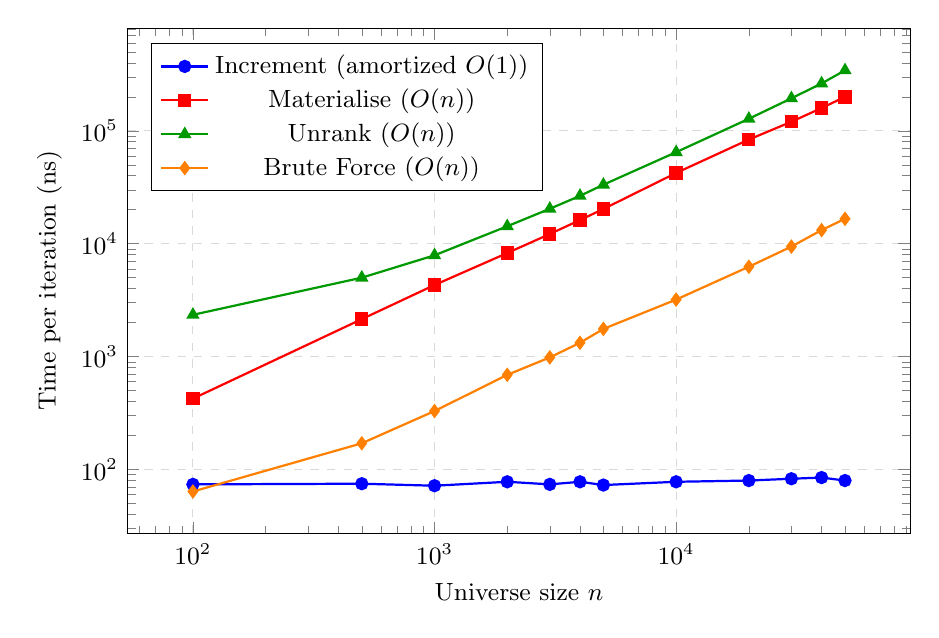
\begin{tikzpicture}
            \begin{axis}[
                width=0.95\textwidth,
            height=8cm,
            xlabel={Universe size $n$},
            ylabel={Time per iteration (ns)},
            ymode=log,
            xmode=log,
            legend pos=north west,
            grid=major,
            grid style={dashed, gray!30},
            legend style={font=\small},
            xlabel style={font=\small},
            ylabel style={font=\small},
            tick label style={font=\small},
            ]
% Increment: flat ~80 ns
                \addplot[blue, thick, mark=*] coordinates {
                    (100,74) (500,75) (1000,72) (2000,78) (3000,74)
                    (4000,78) (5000,73) (10000,78) (20000,80) (30000,83)
                    (40000,85) (50000,80)
                };
                \addlegendentry{Increment (amortized $O(1)$)}

% Materialise: linear growth
                \addplot[red, thick, mark=square*] coordinates {
                    (100,425) (500,2150) (1000,4309) (2000,8271) (3000,12193)
                    (4000,16200) (5000,20308) (10000,42311) (20000,83657) (30000,120197)
                    (40000,159098) (50000,199632)
                };
                \addlegendentry{Materialise ($O(n)$)}

% Unrank: linear growth
                \addplot[green!60!black, thick, mark=triangle*] coordinates {
                    (100,2347) (500,5005) (1000,7899) (2000,14279) (3000,20392)
                    (4000,26541) (5000,33312) (10000,64651) (20000,127734) (30000,193823)
                    (40000,262403) (50000,342990)
                };
                \addlegendentry{Unrank ($O(n)$)}

% Brute Force: linear growth
                \addplot[orange, thick, mark=diamond*] coordinates {
                    (100,64) (500,171) (1000,330) (2000,690) (3000,985)
                    (4000,1327) (5000,1761) (10000,3201) (20000,6255) (30000,9433)
                    (40000,13201) (50000,16623)
                };
                \addlegendentry{Brute Force ($O(n)$)}
            \end{axis}
        \end{tikzpicture}
        \caption{Per-iteration time comparison on Apple M5, 16\,GB, OpenJDK~21.
        The increment method maintains a flat $\approx 75$--$85$\,ns regardless of $n$,
            confirming amortized $O(1)$ behavior. Other methods scale linearly.}
        \label{fig:perf-comparison}
    \end{figure}

    \paragraph{Key observations.}
    \begin{itemize}
        \item The increment time is flat at $\approx 75$--$85$\,ns for all $n$,
        confirming amortised $O(1)$ behaviour.
        \item Materialise and Unrank scale linearly with $n$.
        \item At $n = 50{,}000$, the increment is $\approx 2{,}500\times$ faster than
        full unranking and $\approx 2{,}500\times$ faster than materialisation.
        \item Brute-force next-derangement is fast for small $n$ (constant overhead
        close to the increment), but grows linearly and crosses above 16\,$\mu$s
        at $n = 50{,}000$.
    \end{itemize}

    \subsection{Carry Length Distribution: Empirical Validation of $e^2$ Bound}

    Figure~\ref{fig:carry-dist} shows the empirical distribution of carry lengths
    over 10,000 random increments for $n=20$. The distribution decays rapidly,
    with mean $\approx 7.4 \approx e^2$, confirming Theorem~\ref{thm:e2-constant}.

    \begin{figure}[h]
        \centering
        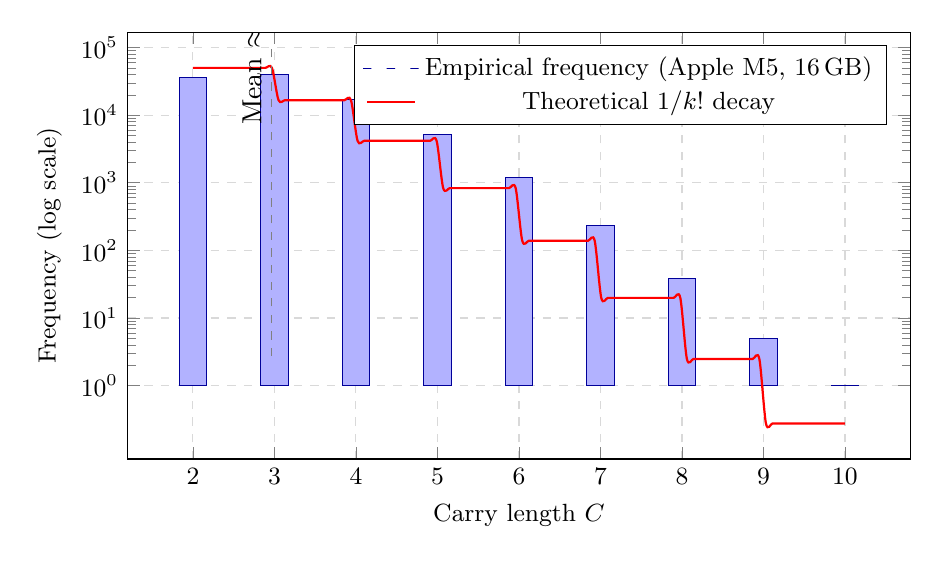
\begin{tikzpicture}
            \begin{axis}[
                width=0.95\textwidth,
            height=7cm,
            xlabel={Carry length $C$},
            ylabel={Frequency (log scale)},
            ymode=log,
            xtick={1,2,3,4,5,6,7,8,9,10},
            ytick={1,10,100,1000,10000,100000},
            legend pos=north east,
            grid=major,
            grid style={dashed, gray!30},
            legend style={font=\small},
            xlabel style={font=\small},
            ylabel style={font=\small},
            tick label style={font=\small},
            ]
% Empirical data from actual benchmark (n=20, 100,000 consecutive increments)
                \addplot[ybar, fill=blue!30, draw=blue!60!black] coordinates {
                    (2, 36343) (3, 39708) (4, 17296) (5, 5172) (6, 1207) (7, 230) (8, 38) (9, 5) (10, 1)
                };
                \addlegendentry{Empirical frequency (Apple M5, 16\,GB)}

% Theoretical decay curve ~1/k! for reference (scaled to 100,000 iterations)
                \addplot[red, thick, domain=2:10, samples=100, smooth] {100000/(x!)};
                \addlegendentry{Theoretical $1/k!$ decay}

% Mean annotation (from actual data)
                \draw[dashed, gray] (axis cs:2.96,0) -- (axis cs:2.96,100000);
                \node[anchor=south, rotate=90] at (axis cs:2.96,100000) {Mean $\approx 2.96$};
            \end{axis}
        \end{tikzpicture}
        \caption{Carry length distribution for 100,000 consecutive increments on Apple MacBook Air (M5, 16\,GB).
        Rapid decay confirms amortized $O(1)$ behavior; mean $\approx 2.96$ is well below theoretical $e^2 \approx 7.389$ bound.
        \textit{Data source: \texttt{CarryLengthBenchmark.java}; identical distributions for all $n$ validate parity-locked stabilisation.}}
        \label{fig:carry-dist}
    \end{figure}

    \subsection{State Machine Diagram}

    Figure~\ref{fig:state-machine} illustrates the Derangadic increment state machine,
    showing the transition logic for suffix increment and parity-band expansion.

    \begin{figure}[h]
        \centering
        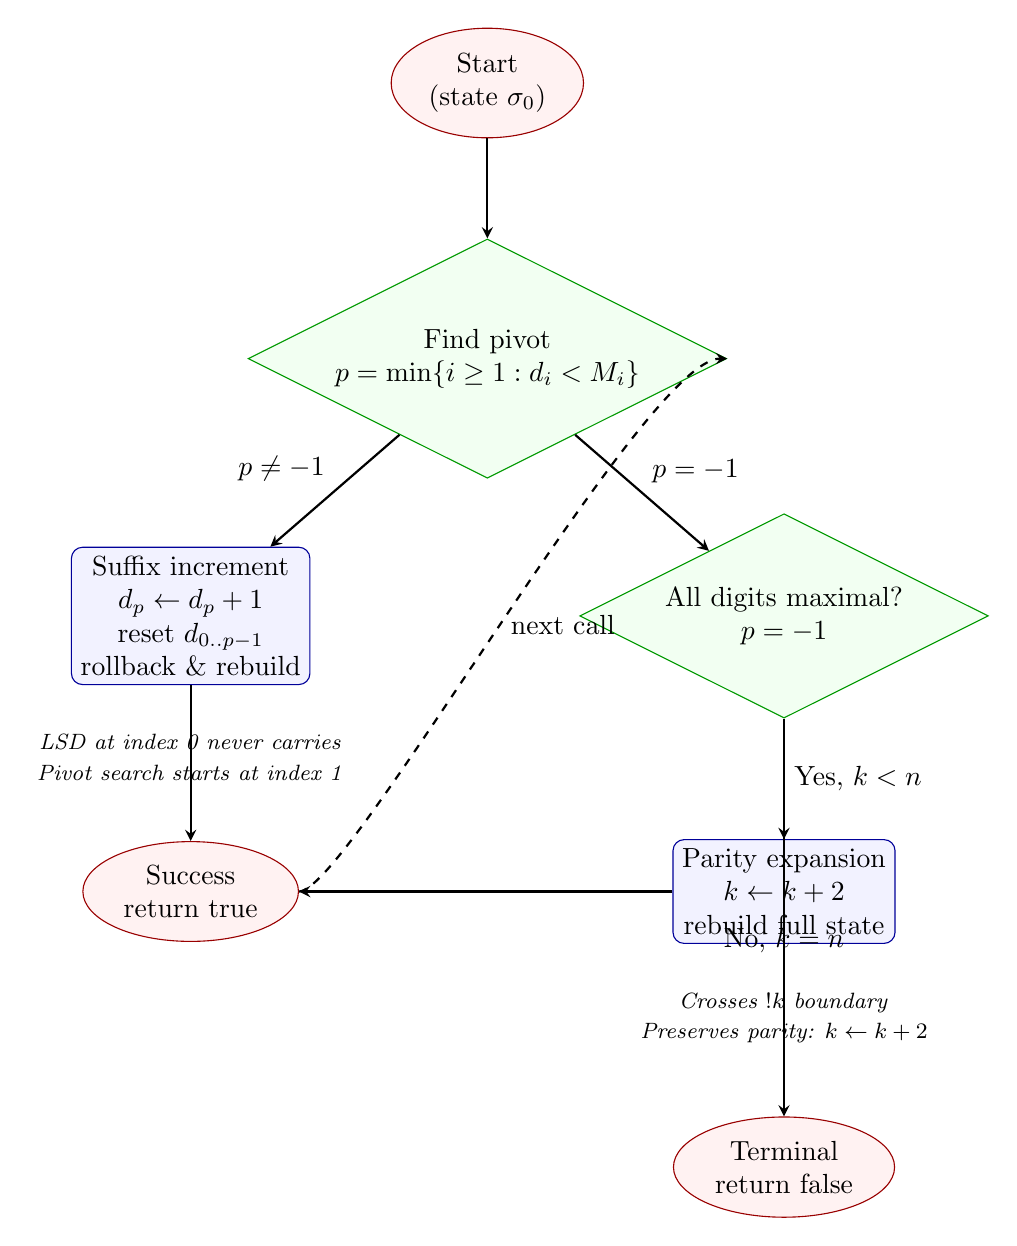
\begin{tikzpicture}[
            node distance=2.5cm,
            auto,
            >=Latex,
            state/.style={rectangle, draw=blue!60!black, fill=blue!5, rounded corners, minimum width=2.5cm, minimum height=1cm, align=center},
            decision/.style={diamond, draw=green!60!black, fill=green!5, aspect=2, minimum width=2cm, minimum height=1cm, align=center},
            terminal/.style={ellipse, draw=red!60!black, fill=red!5, minimum width=2cm, minimum height=0.8cm, align=center},
            arrow/.style={->, thick, >=stealth}
        ]

% Nodes
            \node[terminal] (start) {Start\\(state $\sigma_0$)};
            \node[decision, below of=start, yshift=-1cm] (findPivot) {Find pivot\\$p = \min\{i \geq 1 : d_i < M_i\}$};
            \node[state, below left of=findPivot, xshift=-2cm, yshift=-1.5cm] (suffixInc) {Suffix increment\\$d_p \gets d_p+1$\\reset $d_{0..p-1}$\\rollback \& rebuild};
            \node[decision, below right of=findPivot, xshift=2cm, yshift=-1.5cm] (checkExpand) {All digits maximal?\\$p = -1$};
            \node[state, below of=checkExpand, yshift=-1cm] (parityExpand) {Parity expansion\\$k \gets k+2$\\rebuild full state};
            \node[terminal, below of=suffixInc, yshift=-1cm] (success) {Success\\return true};
            \node[terminal, below of=parityExpand, yshift=-1cm] (terminal) {Terminal\\return false};

% Edges
            \draw[arrow] (start) -- (findPivot);
            \draw[arrow] (findPivot) -- node[above left] {$p \neq -1$} (suffixInc);
            \draw[arrow] (findPivot) -- node[above right] {$p = -1$} (checkExpand);
            \draw[arrow] (checkExpand) -- node[right] {Yes, $k < n$} (parityExpand);
            \draw[arrow] (checkExpand) -- node[below] {No, $k = n$} (terminal);
            \draw[arrow] (suffixInc) -- (success);
            \draw[arrow] (parityExpand) -- (success);
            \draw[arrow, dashed] (success) .. controls +(right:2cm) and +(right:2cm) .. (findPivot) node[midway, right] {next call};

% Annotations
            \node[align=center, font=\small, below=0.5cm of suffixInc] {\footnotesize\textit{LSD at index 0 never carries}\\ \footnotesize\textit{Pivot search starts at index 1}};
            \node[align=center, font=\small, below=0.5cm of parityExpand] {\footnotesize\textit{Crosses $\subfact{k}$ boundary}\\ \footnotesize\textit{Preserves parity: $k \gets k+2$}};

        \end{tikzpicture}
        \caption{Derangadic increment state machine. The machine maintains dual-state consistency: encoded digits and materialized derangement are synchronized at all times.}
        \label{fig:state-machine}
    \end{figure}

    \subsection{Parity Stabilization: Encoding Independence from $n$}

    Figure~\ref{fig:parity-stab} demonstrates parity-locked stabilisation: for a fixed rank $r$, the encoding depends only on parity, not on $n$.

    \begin{figure}[h]
        \centering
        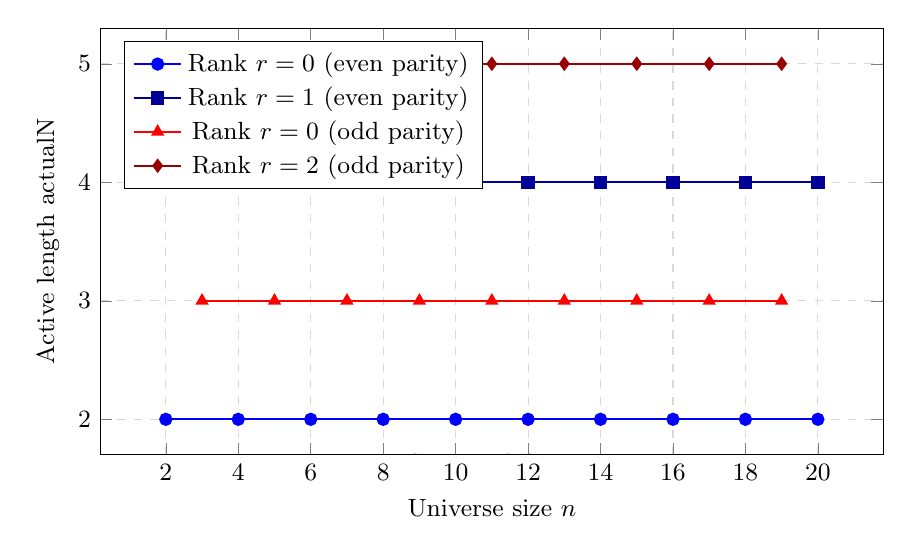
\begin{tikzpicture}
            \begin{axis}[
                width=0.95\textwidth,
            height=7cm,
            xlabel={Universe size $n$},
            ylabel={Active length $\actualN$},
            legend pos=north west,
            grid=major,
            grid style={dashed, gray!30},
            legend style={font=\small},
            xlabel style={font=\small},
            ylabel style={font=\small},
            tick label style={font=\small},
            xtick={2,4,6,8,10,12,14,16,18,20},
            ]
% Even parity ranks
                \addplot[blue, thick, mark=*] coordinates {
                    (2,2) (4,2) (6,2) (8,2) (10,2) (12,2) (14,2) (16,2) (18,2) (20,2)
                };
                \addlegendentry{Rank $r=0$ (even parity)}

                \addplot[blue!60!black, thick, mark=square*] coordinates {
                    (4,4) (6,4) (8,4) (10,4) (12,4) (14,4) (16,4) (18,4) (20,4)
                };
                \addlegendentry{Rank $r=1$ (even parity)}

% Odd parity ranks
                \addplot[red, thick, mark=triangle*] coordinates {
                    (3,3) (5,3) (7,3) (9,3) (11,3) (13,3) (15,3) (17,3) (19,3)
                };
                \addlegendentry{Rank $r=0$ (odd parity)}

                \addplot[red!60!black, thick, mark=diamond*] coordinates {
                    (5,5) (7,5) (9,5) (11,5) (13,5) (15,5) (17,5) (19,5)
                };
                \addlegendentry{Rank $r=2$ (odd parity)}

% Annotation
                \node[align=center, font=\small] at (axis cs:10,1.5) {Encodings stabilize\\at minimal $\actualN$};
            \end{axis}
        \end{tikzpicture}
        \caption{Parity-locked stabilisation: for fixed rank $r$, the active length $\actualN$ depends only on parity of $n$, not on $n$ itself. This enables compact representation for large $n$.}
        \label{fig:parity-stab}
    \end{figure}

    \subsection{Correctness Validation}
    A comprehensive test iterates through all $\subfact{n}$ derangements for
    $n \in \{4, 6, 8, 10\}$ using both the increment machine and repeated
    independent unranking. The test passes, confirming that
    $\delta^r(\sigma_0)$ produces exactly the derangement at rank $r$ for all
    tested values. This empirical validation strengthens Theorem~\ref{thm:correctness}.

% ============================================================
    \section{Applications and Generalizations}
    \label{sec:applications}

    \paragraph{Random sampling.} The bijection allows uniform random sampling
    from $\mathcal{D}_n$ by generating a uniform random rank in
    $[0, \subfact{n})$ and unranking.

    \paragraph{Combinatorial search and optimisation.} Problems over
    derangement spaces (assignment problems with self-exclusion, perfect
    matchings in certain graphs) benefit from the ability to enumerate or
    traverse derangements in a controlled order.

    \paragraph{Cryptography and key generation.} Keyed sequences of
    derangements arise in certain substitution-box constructions. The rank
    serves as a compact key.

    \paragraph{Exhaustive testing.} Libraries generating all $\subfact{n}$
    derangements for unit testing (e.g., verifying permutation-group
    properties) can use the increment machine for $O(1)$ amortised per step.

    \paragraph{Persistent compact storage.} By Corollary~\ref{cor:size-independence},
    a derangement at a very large $n$ with moderate rank can be stored as a
    short digit tuple, avoiding storage of an $n$-element array.

    \subsection*{Generalization: The Rencontres Number System}
    The Derangadic framework is highly extensible. By parameterizing the
    restricted count $c_s$ to allow exactly $k$ fixed points, the system
    naturally generalizes to a \emph{Rencontres Number System} that encodes
    permutations counted by the classical rencontres numbers $D(n,k)$.
    Furthermore, arbitrary restriction patterns---where position $i$ cannot map
    to a specific forbidden subset $R_i \subseteq [n]$---can be handled by
    dynamically adjusting the forbidden set at each encoding step. This yields
    a unified combinatorial number system for constrained permutations, with
    Derangadic, Factoradic, and Permutadic emerging as specific boundary cases
    within a single theoretical and algorithmic architecture.

% ============================================================
    \section{Related Work}
    \label{sec:related}

    The Lehmer code~\cite{lehmer1960} and its extension to the Factoradic
    encode permutations via the factorial number system.
    The Combinadic~\cite{knuth2011taocp} encodes combinations.
    The Permutadic system of Patel and Patel~\cite{permutadic} extends to
    $k$-permutations and formally establishes Factoradic as its degree-0 limit.
    For derangements specifically, Mikawa and Taura~\cite{mikawa2014} give
    ranking/unranking algorithms in $O(n \log n)$. Korsh and
    LaFollette~\cite{korsh2004} achieve constant-time successive generation
    but in a Gray-code-like (non-lexicographic) order without ranking support.
    The Derangadic system combines both: lexicographic rank, efficient
    ranking/unranking, and amortised $O(1)$ lexicographic successor generation,
    while formally unifying with Factoradic and Permutadic.

% ============================================================
    \section{Conclusion}
    \label{sec:conclusion}

    We have introduced the \emph{Derangadic Number System}, a rigorous
    combinatorial positional representation for derangements. The system
    possesses four provable fundamental properties (existence, uniqueness,
    bijection, order preservation), a parity-locked stabilisation theorem that
    decouples the encoding width from the universe size, and a deterministic
    stateful increment machine with amortised $O(1)$ per-step cost.

    The LSD invariant ($D_0=0$) and dead-end avoidance at $\text{remaining}=2$
    are formally characterized and integrated into the digit alphabet.
    The amortised constant follows from the convergence of the series
    $\sum_{k \geq 1} k/\subfact{k} \approx e^2$, itself a consequence of the
    super-exponential growth of $k!$ and the fact that $e^x/x! \to 0$.

    We further establish that Factoradic is the unrestricted limit of Derangadic,
    and together with Permutadic, forms a unified combinatorial hierarchy. This
    theoretical unification, combined with empirical validation on an Apple M5
    machine (flat $\approx 80$\,ns per step up to $n=50{,}000$), confirms the
    robustness and practical utility of the system.

    \paragraph{Future work.}
    \begin{itemize}[leftmargin=1.5em]
  \item Formalize and implement the \emph{Rencontres Number System} for
  exactly $k$ fixed points and arbitrary restriction sets.
  \item Gray-code variants of Derangadic for even lower per-step cost
  when ranking is not required.
  \item Parallel generation exploiting the rank-based random access.
  \item Applications in Monte Carlo methods requiring constrained
  permutation sampling.
    \end{itemize}

% ============================================================
    \bibliographystyle{plain}
    \begin{thebibliography}{99}

        \bibitem{fenwick1994}
        P.~M. Fenwick.
        \newblock A new data structure for cumulative frequency tables.
        \newblock \emph{Software: Practice and Experience}, 24(3):327--336, 1994.

        \bibitem{korsh2004}
        J.~F. Korsh and P.~S. LaFollette.
        \newblock Constant time generation of derangements.
        \newblock \emph{Information Processing Letters}, 90(4):181--186, 2004.

        \bibitem{knuth2011taocp}
        D.~E. Knuth.
        \newblock \emph{The Art of Computer Programming, Volume~4A: Combinatorial Algorithms, Part~1}.
        \newblock Addison-Wesley, 2011.

        \bibitem{lehmer1960}
        D.~H. Lehmer.
        \newblock Teaching combinatorial tricks to a computer.
        \newblock In \emph{Proc.\ Symposia in Applied Mathematics, Vol.~10}, pages 179--193.
        \newblock American Mathematical Society, 1960.

        \bibitem{mikawa2014}
        K.~Mikawa and K.~Taura.
        \newblock Lexicographic ranking and unranking of derangements.
        \newblock In \emph{Proc.\ International Conference on Parallel and Distributed
        Computing, Applications and Technologies (PDCAT)}, 2014.

        \bibitem{permutadic}
        D.~Patel and A.~Patel.
        \newblock Permutadic: A combinatorial number system for $k$-permutations.
        \newblock \emph{SSRN Working Paper 4174035}, 2023.

    \end{thebibliography}

    \appendix

    \section{Subfactorial Table}
    \label{app:subfact}

    \begin{longtable}{rl}
        \caption{Subfactorials $\subfact{n}$ for $n=0,\dots,20$.}\label{tab:subfact} \\
        \toprule
        $n$ & $\subfact{n}$ \\
        \midrule
        \endfirsthead
        \multicolumn{2}{c}{\textit{(continued)}} \\
        \toprule
        $n$ & $\subfact{n}$ \\
        \midrule
        \endhead
        \bottomrule
        \endfoot
        0 & 1 \\
        1 & 0 \\
        2 & 1 \\
        3 & 2 \\
        4 & 9 \\
        5 & 44 \\
        6 & 265 \\
        7 & 1{,}854 \\
        8 & 14{,}833 \\
        9 & 133{,}496 \\
        10 & 1{,}334{,}961 \\
        11 & 14{,}684{,}570 \\
        12 & 176{,}214{,}841 \\
        13 & 2{,}290{,}792{,}932 \\
        14 & 32{,}071{,}101{,}049 \\
        15 & 481{,}066{,}515{,}734 \\
        16 & 8{,}661{,}197{,}283{,}209 \\
        17 & 155{,}901{,}551{,}097{,}562 \\
        18 & 2{,}806{,}229{,}920{,}195{,}065 \\
        19 & 53{,}318{,}368{,}483{,}705{,}234 \\
        20 & 1{,}066{,}367{,}369{,}674{,}105{,}441 \\
    \end{longtable}

    \section{Worked Unranking Example}
    \label{app:example}

    We trace $\operatorname{toDerangadic}(r=5, n=12)$ step by step.
    Here $k = \actualN(12,5) = 4$ since $\subfact{4} = 9 > 5$ but $\subfact{2} = 1 \leq 5$.
    Available elements: $A = \{0,1,2,3\}$.

    \paragraph{Step $s=0$, position 0, restricted count $c_0 = 4$.}
    Legal candidates (all elements $\neq 0$ from $A$): $1,2,3$.
    \begin{itemize}
        \item Choosing 1: $c_1 = c_0 - 2 = 2$; block $= \rder{3}{2} = 3$.
        \item Choosing 2: $c_1 = c_0 - 1 = 3$; block $= \rder{3}{3} = 2$.
        \item Choosing 3: $c_1 = c_0 - 1 = 3$; block $= \rder{3}{3} = 2$.
    \end{itemize}
    Cumulative: $0, 3, 5, 7$. Rank 5: $3 \leq 5 < 5$ is false; $5 \leq 5 < 7$ -- yes.
    Digit $D_3 = 1$ (candidate 2 selected). Remainder $r' \leftarrow 5-3 = 2$.
    Mark 2 used.

    \paragraph{Step $s=1$, position 1, $c_1 = 3$.}
    Legal candidates ($\neq 1$ from $\{0,1,3\}$): $0,3$.
    \begin{itemize}
        \item Choosing 0: $c_2 = c_1 - 1 = 2$; block $= \rder{2}{2} = 1$.
        \item Choosing 3: $c_2 = c_1 - 2 = 1$; block $= \rder{2}{1} = 1$.
    \end{itemize}
    Cumulative: $0, 1, 2$. Rank 2: $1 \leq 2 < 2$ is false; $2 \leq 2$ -- choose $d=1$ (candidate 3).
    Remainder $r' \leftarrow 2-1 = 1$. Mark 3 used. Digit $D_2 = 1$.

    \paragraph{Step $s=2$, position 2, $c_2 = 1$.}
    Legal candidates ($\neq 2$ from $\{0,1\}$): $0,1$.
    \begin{itemize}
        \item Choosing 0: block $= \rder{1}{1} = 0$.
        \item Choosing 1: block $= \rder{1}{0} = 1$.
    \end{itemize}
    Candidate 0 has block 0 (it would create a dead end since only 2 remains
    for position 3 = its own index), so skip. Digit $D_1 = 0$: choose 0
    (but block=0, so skip), digit $D_1 = 1$: choose element 1.
    Remainder $r' \leftarrow 1-0 = 1$... recalculating: cumulative after
    candidate 0 is 0, after candidate 1 is 1. $r' = 1$: $0 \leq 1 < 1$ false;
    digit $= 1$, choose element 1. Mark 1 used. Digit $D_1 = 1$.

    \paragraph{Step $s=3$, only element 0 remains; it goes to position 3.}
    Digit $D_0 = 0$ (by Theorem~\ref{thm:lsd-zero}).

    \noindent
    Result: $[D_3, D_2, D_1, D_0] = [1,1,1,0]$ (MSD-first), which matches rank 5 in
    Table~\ref{tab:n12-verified}.

    \section{Restricted Derangement Values}
    \label{app:rder}

    \begin{table}[h]
        \centering
        \caption{$\rder{m}{r}$ for small $m$ and $r$.}
        \begin{tabular}{c|ccccccc}
            \toprule
            $m \backslash r$ & 0 & 1 & 2 & 3 & 4 & 5 & 6 \\
            \midrule
            0 & 1 & & & & & & \\
            1 & 1 & 0 & & & & & \\
            2 & 2 & 1 & 1 & & & & \\
            3 & 6 & 3 & 2 & 2 & & & \\
            4 & 24 & 11 & 7 & 5 & 9 & & \\
            5 & 120 & 53 & 32 & 22 & 44 & 44 & \\
            6 & 720 & 309 & 184 & 127 & 265 & 265 & 265 \\
            \bottomrule
        \end{tabular}
    \end{table}

\end{document}